%\chapter{Transient Analysis and Deterministic Optimization of Dynamical Systems}
\chapter{Multibody Dynamics and Adjoint Based Deterministic Optimization}
\label{chapter:detapps}
\epigraph{For since the fabric of the universe is most perfect and the
  work of a most wise Creator, nothing at all takes place in the
  universe in which some rule of maximum or minimum does not
  appear.}{Leonard Euler [1707-1783]}

\paragraph*{Introduction.}
The intent of this chapter is to show the physical application of the time marching and adjoint sensitivity framework presented in Chapter~\ref{chapter:adjoint-ode} to design optimization problems in the context of flexible multibody dynamics.
We start with simple dynamical system such as a pendulum and build upon complexity by adding flexible bodies, kinematic constraints and motion actuators. We end this chapter with a rotorcraft optimization application.
%The second-order differential equations in time and are solved without conversion to first-order form.
%The higher-order initial value problems from fields such as chaotic dynamics are also analysed using the proposed framework.

% \section{Aeroelastic oscillator}
% This is an unconstrained two degree of freedom system modeled by the
% following coupled differential equations.

\section{Triple Pendulum}
%
\begin{figure}[h]
  \centering
  \includegraphics[width=0.5\textwidth]{pendulum.pdf}
  \caption{The schematic of the triple pendulum system.}
  \label{fig:pendulum_system}
\end{figure}

\subsection{Analysis Setup}
%This is the first case employing rigid body elements and kinematic constraints.
%
% In this section, we describe the application of the proposed multibody dynamics framework to a triple pendulum system.

Figure~\ref{fig:pendulum_system} shows the triple pendulum system with three rigid bodies which are denoted as $\mathcal{B} = \{A,\,B,\,C\}$ and three kinematic constraints at the points $\mathcal{P} = \{1,\,2,\,3\}$.
The properties of the bodies and the kinematic constraints are listed in Tables~\ref{tab:pendulum_bodies} and~\ref{tab:pendulum_joints}, respectively.
The body axes are chosen such that one of the orthogonal axes are aligned with the geometrical dimensions of the body to simplify the calculation of the inertial properties.
The bodies are assumed to have constant material density.
%
\begin{table}[h]
  \caption{List of bodies in the pendulum system and their properties.}
  \centering
  \begin{tabular}{c c c c c c}
    \toprule
        {Body}    & Type  & Mass & Length & Width & Thickness \\
        \midrule
        A         &  Rigid  & 1.0  & 1.0    & 0.1 & 0.1 \\
        B         &  Rigid  & 2.0  & 2.0    & 0.1 & 0.1 \\
        C         &  Rigid  & 3.0  & 3.0    & 0.1 & 0.1 \\
        \bottomrule
  \end{tabular}
  \label{tab:pendulum_bodies}
\end{table}
%
\begin{table}[h]
  \caption{List of kinematic constraints in the pendulum system and their properties.}
  \centering
  \begin{tabular}{c c c}
    \toprule
        {Joint} & Type  & Components\\
        \midrule
        1  & Spherical & $F_I$ and body A \\
        2  & Revolute (hinge)  & Bodies A and B \\
        3  & Revolute (hinge) & Bodies B and C \\
        \bottomrule
  \end{tabular}
  \label{tab:pendulum_joints}
\end{table}

% Each body contributes twelve degrees of freedom to the multibody system resulting from the position vector, velocity, angular velocity and Euler angles.
% Each kinematic constraint contributes six degrees of freedom corresponding to the reaction forces and torques.
% As a result, there are 54 state variables associated with the rigid-body motion of the triple pendulum.
%
\begin{figure}[h!]
  \centering
  \includegraphics[width=0.75\textwidth]{full_pendulum_motion}
  \caption{Motion of the triple pendulum over the first 3 seconds.}
  \label{fig:pendulum_time_lapse}
\end{figure}

\subsection{Dynamics}
Figure~\ref{fig:pendulum_time_lapse} shows the timelapse of motion of the bodies in the system over a duration of three seconds.
The effect of the revolute joint can be seen where the adjacent bodies in the joint are constrained to rotate about a locally-aligned axis.
Figure~\ref{fig:pendulum_energy} shows the changes in the potential and kinetic energies of the system over a 10 second time interval.
Since non-conservative forces are not modeled, such as joint friction, the sum of the potential and kinetic energy should remain constant.
Figure~\ref{fig:pendulum_energy:a} illustrates the complementary trend of energy transfer between kinetic and potential energies.
However, the limited numerical accuracy of the time integration scheme introduces an energy defect that can grow over time.
To assess this error, Figure~\ref{fig:pendulum_energy} shows the energy loss over the same time period. Note that over the entire simulation, the energy loss is about $2 \times 10^{-3}$\,J.
%
\begin{figure}[H]
  \centering
  \begin{subfigure}{0.48\linewidth}
    \includegraphics[width=\textwidth]{pendulum_energy.pdf}
    \caption{Kinetic and potential energy}
    \label{fig:pendulum_energy:a}
  \end{subfigure}
  \begin{subfigure}{0.48\linewidth}
    \includegraphics[width=\textwidth]{pendulum_energyloss.pdf}
    \caption{Total energy loss over the time interval}
    \label{fig:pendulum_energy:b}
  \end{subfigure}
  \caption{Plot of the potential, kinetic and total energies with time
    for the pendulum system.}
  \label{fig:pendulum_energy}
\end{figure}

\subsection{Adjoint Gradients}
\begin{figure}[h!]
  \centering
  \includegraphics[width=0.9\textwidth]{pendulum_cs_verify.pdf}
  \caption{Gradient verification study with the complex-step method using step sizes of $10^{-4}$, $10^{-8}$, $10^{-12}$, and $10^{-16}$.}
  \label{fig:pendulum-verify}
\end{figure}
Figure~\ref{fig:pendulum-verify} shows a complex-step verification of the adjoint-gradient computed using BDF method.
The verification study compares the derivative of Kreisselmeier--Steinhauser~\citep{original-KS-paper:1979,Kennedy:2015:ks-paper, Kennedy:2015:adaptive-ks} aggregation of velocity with respect to a series of design variables consisting of initial configuration variables and inertial properties.
The KS function approximates the maximum velocity achieved over the time interval of the simulation.
%The complex-step method does not suffer from subtractive cancellation, which enables the use of very small step sizes, producing highly accurate gradient estimates.
Each component of the gradient exhibits a relative accuracy on the order of $10^{-12}$, illustrating near machine precision accuracy of all gradients.

\section{Trebuchet (Catapult)}
%This is the second case employing fully rigid bodies and kinematic constraints.
Trebuchets have been used for warfare from fifth century B.C till medieval times.
In this section we study the multibody dynamics of trebuchet and apply it to an optimization problem of achieving maximum range of the projectile.
The trebuchet works to transfer the potential energy of the counterweight to impart kinetic energy to the projectile mass.

\subsection{Analysis Setup}
\begin{figure}[H]
  \centering
  \includegraphics[width=0.6\textwidth]{trebuchet_without_support.pdf}
  \caption{The schematic of the trebuchet system.}
  \label{fig:trebuchet_schematic}
\end{figure}
The trebuchet is created using five bodies given by $\mathcal{B} = \{A,\,B,\,C,\,D,\,E\}$, and five kinematic constraints labeled $\mathcal{P} =\{1,\,2,\,3,\,4,\,5\}$ as shown in Figure~\ref{fig:trebuchet_schematic}.
The kinematic constraints at points 1, 2 and 3 are revolute, while the other joints at points 4 and 5 are modeled as spherical.
The whole trebuchet assembly rotates about the axle at point 5.
The body axes are chosen to enable convenient calculation of inertial properties.
Table~\ref{tab:trebuchet_bodies} contains the list of bodies and their geometric/material properties.
% The trebuchet arm, body C, is not a uniform geometry and representative values are tabulated.
% The rigid part of the multibody dynamic system contains 90 unknowns, 60 kinematic and dynamic variables and 30 unknown internal reaction forces and torques.
\begin{table}[h!]
  \caption{List of bodies in the trebuchet system and their properties.}
  \centering
  \begin{tabular}{c c c c c c}
    \toprule
        {Body}    & Name             & Density  &Length & Width & Thickness \\
        \midrule
        A         &  Counter weight  & 25   & 4  & 4 & 1 \\
        B         &  Connecting link & 10   & 0.5  & 0.5 & 2 \\
        C         &  Arm             & 2    & 20 & 0.5 & 2 \\
        D         &  Projectile link & $10^{-2}$ & 0.2  & 0.5 & 6 \\
        E         &  Projectile      & $10^{-2}$ & 1  & 1 & 1 \\
        \bottomrule
  \end{tabular}
  \label{tab:trebuchet_bodies}
\end{table}
Figure~\ref{fig:trebuchet_time_lapse} depicts the motion of the trebuchet system obtained using BDF method.
The trebuchet arm starts from a horizontal orientation and reaches a near vertical position as it rotates about the axle.
Note that the axle is not shown explicitly.
The angular momentum of the swinging motion generated by the counterweight is transferred as linear momentum to the projectile mass through the arm and projectile link.
\begin{figure}[h!]
  \centering
  \includegraphics[width=0.95\textwidth]{trebuchet_time_lapse.png}
  \caption{Motion of the trebuchet}
  \label{fig:trebuchet_time_lapse}
\end{figure}
Figure~\ref{fig:trebuchet_energy} shows the kinetic and potential energy in the trebuchet system over the time history of the simulation.
During the motion, the potential energy of the system, stored primarily in the counterweight is transferred to kinetic energy.
The total energy of the system is conserved, since no non-conservative forces are modeled.
The time integration error produces a small change of less than $3\times 10^{-2}$\,J in the total energy in the system, as shown in Figure~\ref{fig:trebuchet_energy}.
This energy loss can be reduced by utilizing a smaller time integration step size.
\begin{figure}[h]
  \centering
  \begin{subfigure}[b]{0.7\linewidth}
    \includegraphics[width=1.0\textwidth]{trebuchet_energy.pdf}
    \caption{Kinetic and potential energy}
    \label{fig:trebuchet_energy:a}
  \end{subfigure}
  \begin{subfigure}[b]{0.7\linewidth}
    \includegraphics[width=1.0\textwidth]{trebuchet_energyloss.pdf}
    \caption{Total energy loss over the time interval}
    \label{fig:trebuchet_energy:b}
  \end{subfigure}
  \caption{Plot of the potential, kinetic and total energies with time for the trebuchet system.}
  \label{fig:trebuchet_energy}
\end{figure}

\subsection{Trebuchet optimization}
%In this section, we present the results from the optimization of the trebuchet system described above.
The objective of optimization problem is to maximize projectile range, which is estimated using the kinematics of the projectile motion under gravity.
The precise release point of the projectile is not calculated.
Instead, we use the optimal release point by taking the maximum of the projectile range if it were released at any time during the entire trebuchet motion.
We estimate this maximum range using the KS function, in a similar manner to the maximum velocity function described above.
We also impose a constraint that the projectile must clear a barrier of specified height at a location down range along the path of the projectile.
%This optimization problem is solved using ParOpt~\citep{Kennedy:2015:SciTech}, an in-house interior-point optimization algorithm developed for large-scale optimization problems.
The present trebuchet problem consists of six design variables and one constraint.
The six design variables consist of the mass of the different components within the trebuchet system and an initial condition variable governing the release height of the counterweight.
\begin{figure}[h!]
  \centering
  \begin{subfigure}{0.495\textwidth}
    \centering
    \includegraphics[width=\textwidth]{trebuchet_time_lapse_first_iter.png}
    \caption{Initial design}
  \end{subfigure}
  \begin{subfigure}{0.495\textwidth}
    \centering
    \includegraphics[width=\textwidth]{trebuchet_time_lapse_final_iter.png}
    \caption{Optimized design}
  \end{subfigure}
  \caption{Figure illustrating the initial and final trebuchet designs.}
  \label{fig:trebuchet-design}
\end{figure}
Figure~\ref{fig:trebuchet-design} shows the initial and optimized trebuchet designs.
Note that the counterweight release height is unconstrained at the final design point.
The release height is selected such that the motion of the counterweight is synchronized with the arm and projectile motion to achieve maximum velocity at the release point.

\section{Four-Bar Mechanism}
\subsection{Analysis Setup}
\begin{figure}[H]
  \centering
  \includegraphics[width=0.99\textwidth]{four_bar_example_diagram.pdf}
  \caption{The four-bar mechanism problem used for dynamics verification of TACS.}
  \label{fig:fourbar-problem}
\end{figure}
%A partial verification of the governing equations implemented within the framework is performed against the four-bar mechanism problem reported by~\citet{BauchauBenchmark2016}.
Figure~\ref{fig:fourbar-problem} illustrates the setup of the four-bar mechanism (see \citet{BauchauBenchmark2016}).
Three bars $AB$, $BC$ and $CD$ of the mechanism are joined together using revolute connections.
An imaginary fourth bar exists in the mechanism between the points $A$ and $D$.
The revolute joints at the points $A$, $B$, and $D$, have an axis of rotation that is perpendicular to the plane of the mechanism.
The revolute joint at point $C$ is misaligned by an angle of $5^{\circ}$, rotated about the direction of the bar $CD$.
Bars $AB$ and $BC$ are of the same cross-section, while bar $CD$ has a smaller and more flexible cross section.
The bars in the mechanism are modeled using quadratic beam elements that are derived from Timoshenko beam theory.
% The beam element is implemented using a geometrically exact formulation that captures full rigid rotations and translations, and provides discretely objective strains.
The rotation of bar $AB$ about point $A$ of the mechanism is driven at an angular rate of $\Omega_3 = 0.6$\,rad/s.

\subsection{Motion and Internal Forces}
% Shear locking is avoided through the use of a mixed interpolation of tensorial components (MITC) treatment of the transverse shear strains.
\begin{figure}[h!]
  \centering
  \begin{subfigure}{0.48\linewidth}
    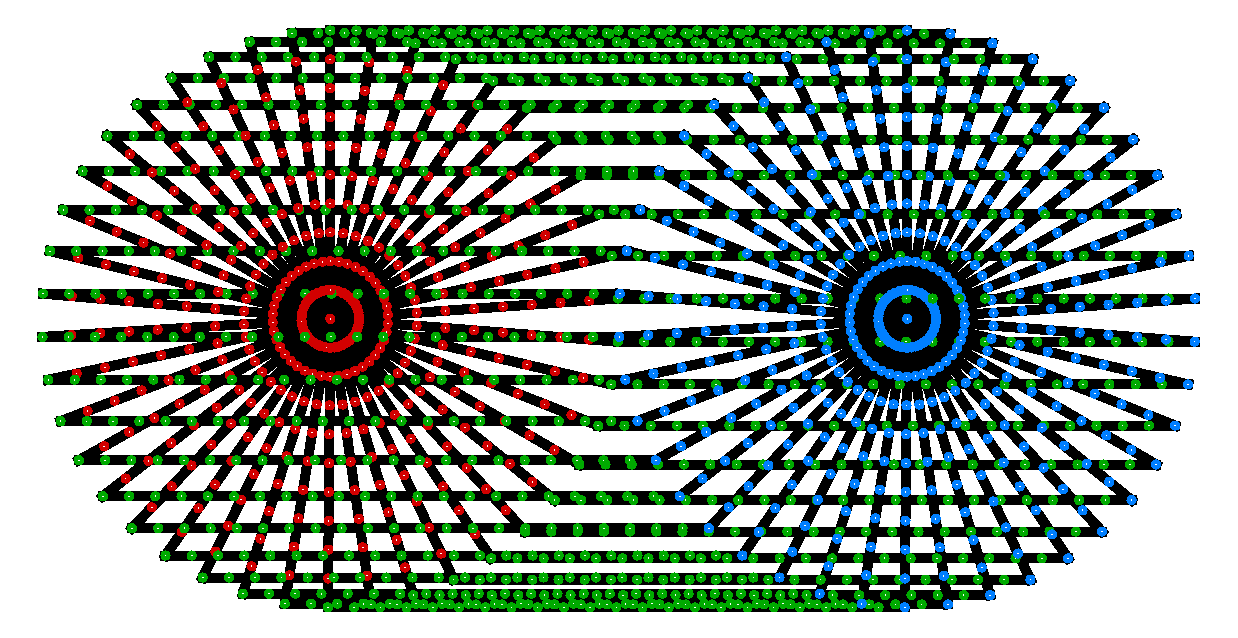
\includegraphics[width=\textwidth]{fourbar_fullmotion.eps}
  \end{subfigure}
  \begin{subfigure}{0.48\linewidth}
    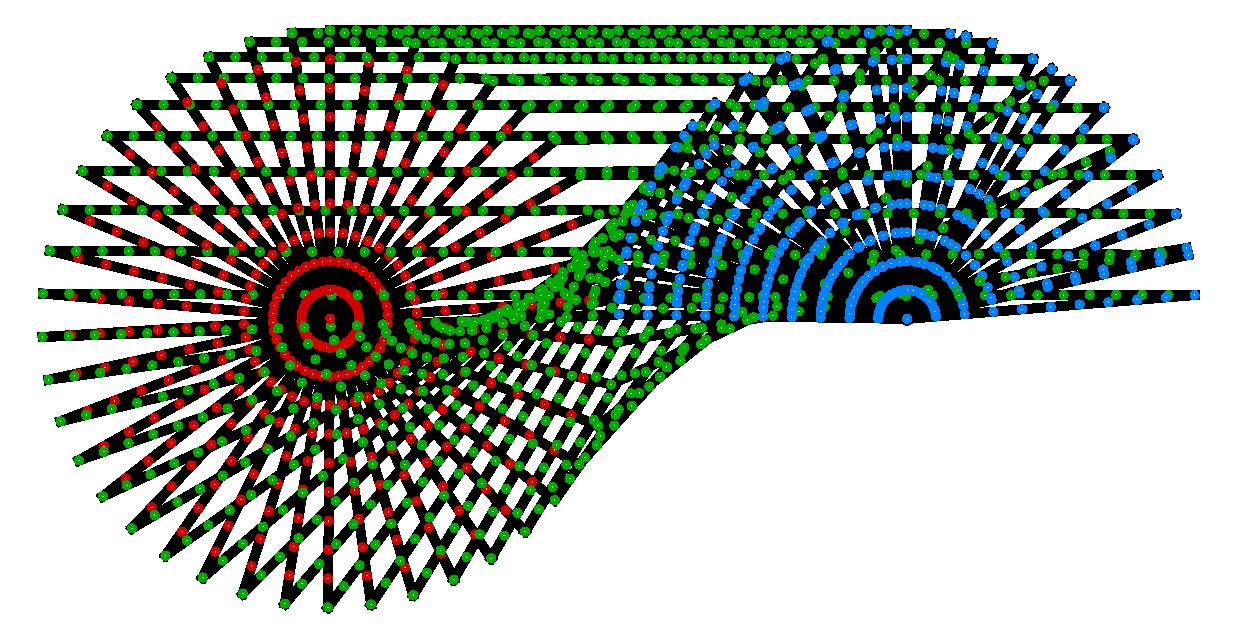
\includegraphics[width=\textwidth]{fourbar_halfmotion.eps}
  \end{subfigure}
  \caption{The time evolution of flexible four-bar mechanism}
  \label{fig:fourbar-motion}
\end{figure}
When the bars are rigid, the four-bar mechanism locks and motion is inhibited. However, when the bars are modeled as flexible, motion becomes possible since the bars can bend to overcome the locking behavior.
The motion of the four-bar mechanism is illustrated in Figure~\ref{fig:fourbar-motion} as a time lapse.
If joint C were not misaligned, the bars would rotate in phase. However, due to the presence of misalignment, the third bar never completes a full rotation, while the first bar drives the motion.
\begin{figure}[h!]
  \centering
  \includegraphics[width=\textwidth]{TACS_dymore_comparison_four_bar.pdf}
  \caption{Comparison of TACS and Dymore~\cite{BauchauBenchmark2016} predictions of force and bending moment in bar $AB$ at mid-span.}
  \label{fig:fourbar-forces}
\end{figure}
Figure~\ref{fig:fourbar-forces} shows a comparison of the axial
force and bending moment in bar $AB$ at the mid-span compared with the
same predictions using Dymore~\citep{BauchauBenchmark2016}. The force
and moment predictions can be seen to be in excellent agreement for
this benchmark problem.

\section{Rotorcraft Hub Dynamics}

%The intent of this section is to demonstrate the suitability of the proposed flexible multibody dynamics framework for analysis and design of rotorcraft models that combine rigid and flexible components as well as kinematic constraints.
% For this purpose, a representative rotor hub configuration is considered for study.
Typical rotorcraft hub assemblies fall under teetering, fully-articulated, hingeless and bearingless categories.
These types differ in the mechanism used to achieve desired flight modes, such as hover or forward flight, and maneuvers, such as roll, pitch and yaw.
To achieve these desired flight modes, the control mechanism must impart collective and cyclic control inputs to the blades through the swashplate driven by the push rods.
The hub and control chain dynamics are a central part of the rotorcraft flight control system and must be accurately modeled to achieve good performance prediction.

\subsection{Model Description}
%Figure~\ref{fig:rotor_assembly_model}
\begin{figure}[h]
  \centering
  \includegraphics[width=\linewidth,trim={4pt 4pt 1.15in 4pt},clip]{rotor_assembly_model_labeled.png}
  \caption{The baseline structural model of rotorcraft hub assembly with its parts labeled.}
  \label{fig:rotor_assembly_model}
\end{figure}
The control chain used for changing the pitch of rotor blades via appropriate inputs to the swashplate is investigated as the motion of interest.
The representative four-bladed rotor hub assembly model used for this application is shown in Figure~\ref{fig:rotor_assembly_model}.
The model consists of rigid bodies, kinematic constraints, flexible bodies and actuators.
The four rotor blades are modeled as flexible using shell elements whereas the remaining parts are modeled as rigid bodies.
The kinematic constraints and actuators used in the rotor assembly are listed in Table~\ref{tab:constraints_actuators}.
The push rods are connected to translational actuators that feed time dependent periodic motions, given by $u(t) = u_0 \sin(\Omega_t t)$, where $\Omega_t$ is the assumed translational control signal frequency.
This driven motion will be used as the basis for the study of different rotorcraft simulation scenarios in the examination of the rotor hub dynamics.
The central shaft is connected to a rotational driver with a angular rate of $\Omega_r=109.12$\,rad/s.
This structural model contains a total of $28,640$ degrees of freedom.
The geometric modeling and meshing parametrization of rotor hub parts is performed using the open-source program GMSH~\cite{Geuzaine2009}.
The inertial properties are obtained directly from the geometry of each part.
\begin{table}[!h]
  \caption{List of constraint types and motion actuators associated with different bodies in hub assembly model.}
  \centering \scalebox{0.99}{
    \begin{tabular}{lcc}
      \toprule
      \textbf{Constraint/Actuator}           & \textbf{Part 1}    & \textbf{Part 2}  \\
      \midrule
      Rotational actuator    & shaft & -- \\
      \midrule
      Translational actuator & push rod & -- \\
      \midrule
      Spherical constraint   & lower swashplate & sphere \\
      Spherical constraint   & upper swashplate & pitch link \\
      Spherical constraint   & pitch link  & pitch horn \\
      Spherical constraint   & lower swashplate  & pitch rod \\
      Spherical constraint   & lower swashplate  & upper push link \\
      \midrule
      Revolute constraint    & lower swashplate & upper swashplate \\
      Revolute constraint    & shaft & pitch horn \\
      Revolute constraint    & baseplate & lower push link \\
      Revolute constraint    & lower push link & upper push link \\
      \midrule
      Cylindrical constraint & sphere & shaft \\
      \midrule
      Fixed constraint       & baseplate & -- \\
      \bottomrule
    \end{tabular}
  }
  \label{tab:constraints_actuators}
\end{table}

\subsubsection{Dynamics}\label{sec:dynamics}
\begin{figure}[!h]
  \centering
  \begin{subfigure}{0.49\linewidth}
    \includegraphics[width=\textwidth,trim={4pt 4pt 4pt 4pt},clip]{zdisplacement_collective_contour.png}
    \caption{collective}
  \end{subfigure}
  \begin{subfigure}{0.49\linewidth}
    \includegraphics[width=\textwidth,trim={4pt 4pt 4pt 4pt},clip]{zdisplacement_longitudinal_contour.png}
    \caption{longitudinal cyclic}
  \end{subfigure}
  \begin{subfigure}{0.49\linewidth}
    \includegraphics[width=\textwidth,trim={4pt 4pt 4pt 4pt},clip]{zdisplacement_lateral_contour.png}
    \caption{lateral cyclic}
  \end{subfigure}
  \caption{Contour plots showing the vertical displacement of bodies
    during the motion in millimeters.}
  \label{fig:displacement_three_motions}
\end{figure}

The rotor hub apparatus is studied for $(a)$ collective $(b)$ longitudinal cyclic and $(c)$ lateral cyclic pitch control imparted through the three push rods at $90^\circ,180^\circ$ and $270^\circ$ from a horizontal reference axis.
These conditions are summarized in Table~\ref{tab:actuator_inputs}.
The corresponding time evolution of the configuration of the rotor assembly is simulated using two-stage, third-order diagonally implicit Runge--Kutta method employing a time step size corresponding to $1^\circ$ per step at the angular rate $109.12$~rad/s.
\begin{table}
  \caption{Sinusoidally modulated control amplitudes supplied to the
    push rods to produce different flight scenarios. }
  \centering \scalebox{1.0}{
    \begin{tabular}{p{4cm}|lccc}
      \toprule
      \textbf{Control}                     & \textbf{Motion} & \textbf{Push rod 1}        & \textbf{Push rod 2}       & \textbf{Push rod 3} \\
      \midrule
      Collective blade pitch control            & vertical         & $ 0.050 \sin(\Omega_t t)$ & $ 0.050 \sin(\Omega_t t)$ & $ 0.050 \sin(\Omega_t t)$ \\
      Longitudinal cyclic blade pitch control   & forward/pitch    & $ 0.025 \sin(\Omega_t t)$ & $ 0.025 \sin(\Omega_t t)$ & $ 0.050 \sin(\Omega_t t)$ \\
      Lateral cyclic blade pitch control        & sideways/roll    & $ 0.025 \sin(\Omega_t t)$ & $ 0.050 \sin(\Omega_t t)$ & $ 0.025 \sin(\Omega_t t)$ \\
      \bottomrule
    \end{tabular}
  }
  \label{tab:actuator_inputs}
\end{table}
%%
%%
Figure~\ref{fig:displacement_three_motions} presents the hub assembly at different time instances for each flight scenario listed in Table~\ref{tab:actuator_inputs}.
The contours illustrate the tilting of the swashplate mechanism that produces a pitching motion for each of the blades.
In the collective case, the blades attain equal blade pitch, which would produce a net upward aerodynamic force during flight.
In the longitudinal and lateral cyclic cases, the pitch of the blades varies as a function of the azimuthal angle and would produce longitudinal and lateral aerodynamic moments during flight.
Therefore, this model combined with the control actuation inputs, can represent different flight scenarios and readily lends itself to a multiscenario optimization case which will be demonstrated later in this section.


\subsection{Adjoint Gradient Verification}
Figure~\ref{fig:rotor-dirk-grad-verify} shows the absolute difference between the adjoint derivatives and the complex-step derivatives on the vertical axis for twelve test functionals indexed on the horizontal axis, for different orders of the DIRK time integration
method.
\begin{figure}[!h]
  \centering
  \includegraphics[width=0.6\textwidth]{rotorcraft-dirk-gradient-verification.pdf}
  \caption{Complex-step verification of the DIRK adjoint formulation of different orders of accuracy
    with 12 functionals with a perturbation size $\delta=10^{-16}$.}
  \label{fig:rotor-dirk-grad-verify}
\end{figure}
%The verification of adjoint formulation presented in Section~\ref{sec:theory} is performed using the complex-step derivative approximation technique.
%The complex-step estimate is obtained by perturbing the input to a function by a complex perturbation as follows
%\begin{equation}\label{eqn:complex-step}
%  \dfrac{d {f}}{d \mb{\xi}_i} = \dfrac{\operatorname{Im}\left(f(\mb{\xi}_{i} + i \delta)\right)  }{\delta} + \mathcal{O} (\delta^2),
%\end{equation}
%where the design variable component $\mb{\xi}_{i}$ is perturbed by $i\,\delta$.
%The complex-step method~\eqref{eqn:complex-step} is second-order accurate, such that the truncation error decreases quadratically with a reduction in perturbation size~\citep{Squire:1998:UCV, Martins:2003:CSD}.
%However, unlike finite-difference method, the complex-step method does not suffer from subtractive cancellation, which enables the use of very small perturbation step sizes to produce highly accurate derivative estimates.
The functionals used for this verification are the structural mass (index 1), the average structural compliance (index 2), the KS aggregates of the von Mises failure criterion (indices 3 and 4), and the induced exponential aggregates~\citep{Kennedy:2015:ks-paper} of the von Mises failure criterion (indices 5 to 12).
Table~\ref{tab:derivative_comparison} shows the magnitude of discrete adjoint sensitivities along with corresponding
complex-step sensitivities.
The digits in boldface represent the entries differing from the complex-step method.
  \begin{table}[!h]
    \caption{Comparison of complex-step and discrete adjoint derivatives for fourth-order DIRK with a perturbation size $\delta=10^{-16}$.}
    \centering \scalebox{1.0}{
      \begin{tabular}{lcc}
        \toprule
        \textbf{Functional} & \textbf{Complex-step}    & \textbf{Adjoint}  \\
        \midrule
        Structural Mass                        & 250.0000000000000       &   249.9999999999999 \\
        Compliance                             & -0.008903780405108      &  -0.0089037804\textbf{57068} \\
        KS (discrete)                          & -2.510549172940552      &  -2.51054917\textbf{3663148} \\
        KS (continuous)                        & -2.505178929745161      &  -2.5051789\textbf{30486006} \\
        Induced (exponential)                  & -2.511154336312865      &  -2.51115433\textbf{7069819} \\
        Induced (discrete exponential)         & -2.516692488940226      &  -2.51669248\textbf{9679126} \\
        Induced (discrete exponential squared) & -0.002788026920568      &  -0.0027880269\textbf{30265} \\
        Induced (exponential squared)          & -0.002762476355788      &  -0.0027624763\textbf{65353} \\
        Induced (power)                        & -4.676554025570486      &  -4.67655402\textbf{8759453} \\
        Induced (discrete power)               & -4.715417147892726      &  -4.7154171\textbf{51435161} \\
        Induced (power squared)                & -0.006574319319522      &  -0.0065743193\textbf{41451} \\
        Induced (discrete power squared)       & -0.006679489586803      &  -0.006679489\textbf{609466} \\
        \bottomrule
      \end{tabular}
    }
    \label{tab:derivative_comparison}
  \end{table}
From Table~\ref{tab:derivative_comparison} and Figure~\ref{fig:rotor-dirk-grad-verify} it can be seen that the adjoint-based derivative exhibits an accuracy of 8 to 14 significant digits for different functionals.
Thus, the adjoint-based gradient evaluation capability achieves sufficient accuracy for gradient-based optimization.

\subsection{Rotorcraft Optimization Demonstration}
The rotorcraft hub is now subject to gradient-based design optimization including all three analysis scenarios (flight-modes) described above.

\subsubsection{Optimization Problem}
The objective of this optimization case is to minimize the mass of the of the rotor blades subject to stress constraints such that the von Mises failure ratio aggregated in space and time domains does not exceed $25\%$ of maximum allowable value.
A mass objective is chosen since more realistic rotor design objectives require multidisciplinary design criteria that cannot be evaluated without a coupled aeroelastic simulation.
The design variables consist of the thicknesses of 48 spanwise panels modeling the rotor blades.
Note that the thickness is constant in the chordwise direction.
The cross-sectional geometry is held constant throughout the span for this demonstration case.
Smoothness requirements are imposed such that thicknesses of successive spanwise panels do not change more than $1$\,mm.
The optimization problem is stated mathematically as follows:
\begin{equation}
  \begin{aligned}
    & \underset{\mb{\xi}}{\text{minimize}} &  & \mathrm{mass} = m(\mb{\xi}), &&\\
    & \text{subject to}            &  & \bar{g}^k(\mb{\xi}) = \xi_k - \xi_{k+1} \le 1\,\text{mm} , && \forall k = 1,\ldots\,\mathrm{47}, & \quad \mathrm{(smoothness~requirement)}\\
    &                              &  & \bar{g}^k(\mb{\xi}) = \xi_{k+1}- \xi_{k} \le 1\,\text{mm} , && \forall k = 1,\ldots\,\mathrm{47},  & \quad \mathrm{(smoothness~requirement)}\\
    &                              &  & \bar{g}^k(\mb{\xi}) = 1 - 4.0\frac{\sigma_{ks}^k}{\sigma_{max}^k}\ge 0, && \forall k = 1,\ldots\,3,  & \quad \mathrm{(stress~constraint)}\\
    & \text{bounds}                &  & 10\,\text{mm} \le \mb{\xi} \le 20\,\text{mm}.
  \end{aligned}
\end{equation}
Each blade is assigned the same set of design variables so that all blades are identical during design.
The time dependent analysis and gradient evaluation for each of the three cases are performed in parallel using five processors.
Both the mass objective and the smoothness constraints are independent of the structural state variables and their gradients are obtained analytically using straightforward differentiation.
The time dependent adjoint formulation developed in this work is used to evaluate the three stress constraint gradients.
The optimization problem with 48 design variables, 3 stress constraints from each flight scenario, and 94 smoothness constraints, is solved using the SLSQP optimizer within the python package pyOpt~\cite{Perez:2011:PYOPT}.

\subsubsection{Optimization Results}
\paragraph*{Optimization History:}
Figure~\ref{fig:feasibility} shows the optimization convergence history.
The optimization took 73 iterations starting from an initial design of $2$\,cm thickness throughout, to converge to infeasibility and optimality tolerance of $10^{-4}$.
Note that the mass and stress constraint infeasibilities are normalized with respect to their values at the initial design.
The mass of the blades (shown in red) decreases immediately from the starting point and stays nearly constant throughout the rest of optimization.
The stress constraint imposed on the lateral blade pitch flight scenario (shown in green) becomes feasible after about 50 iterations.
Finally the stress constraints on longitudinal cyclic (shown in orange) and collective pitch (shown in blue) are satisfied near the termination of optimization algorithm.
The optimization produced a design that has all three stress constraints active.
The optimizer required 222 function evaluations and 88 gradient evaluations.
On average, the forward analysis and gradient evaluation took 33 and 8 minutes, respectively, on five processors.
\begin{figure}[H]
  \centering
  \includegraphics[width=0.99\linewidth]{rotorcraft-opthistory.pdf}
  \caption{History of optimization showing the changes in normalized
    constraint infeasibility and objective values.}
  \label{fig:feasibility}
\end{figure}

\paragraph*{Optimized Design:}
\begin{figure}[h]
  \centering
  \includegraphics[width=0.99\linewidth]{thickness_comparison.png} %{opt_thickness_contour.eps}
  \caption{Comparison of thickness of initial (top) and optimized
    (bottom) designs in millimeters.}
  \label{fig:opt_thickness_contour}
\end{figure}
The final blade design thickness distribution produced by the optimizer is shown in Figure~\ref{fig:opt_thickness_contour}.
Since the blades have identical design variables, only the optimized thickness from one blade is shown.
The optimizer reduced the mass by decreasing the blade thicknesses towards the tip.
The panel thickness gradually decreases along the span until it reaches the lower bound at the tip, thereby reducing the stress at the root.
The gradual variation of panel thickness is a result of enforcing the smoothness constraints in the problem formulation.
Figure~\ref{fig:lambda_comparison} compares the instantaneous stress normalized by design stress in the blades after one full rotation.
\begin{figure}[!h]
  \centering
  \begin{subfigure}{0.99\linewidth}
    \includegraphics[width=\textwidth,trim={2pt 1pt 2pt 1pt},clip]{collective_initopt_normalized_lambda.png}
    \caption{collective}
  \end{subfigure}  \begin{subfigure}{0.99\linewidth}
    \includegraphics[width=\textwidth,trim={2pt 1pt 2pt 1pt},clip]{longitudinal_initopt_normalized_lambda.png} %{longitudinal_lambda_init_opt.png}
    \caption{longitudinal cyclic}
  \end{subfigure}
  \begin{subfigure}{0.99\linewidth}
    \includegraphics[width=\textwidth,trim={2pt 1pt 2pt 1pt},clip]{lateral_initopt_normalized_lambda.png}
    \caption{lateral cyclic}
  \end{subfigure}
  \caption{Comparison of normalized stress failure ratios of initial (left) and optimized (right) blades for different flight scenarios at $360^\circ$ azimuth.}
  \label{fig:lambda_comparison}
\end{figure}
The optimized stresses are lower for all three flight scenarios.
The optimizer thickens the shell elements near the root of the blade that experience higher stress to comply with the stress requirements.
In addition, there are notable differences in stress distribution patterns between each flight scenario, which is anticipated from the differences in dynamics.

% \section{Chaotic Higher-Order systems}

\paragraph*{Summary.}
In this chapter, we presented applications of the implicit solution methods and adjoint framework on problems from flexible multibody dynamics.
For the rotorcraft optimization application, high-fidelity structural dynamics, efficient sensitivity analysis using the adjoint method, along with the  parallel processing capabilities have effectively reduced the optimization time.
